% =============================================================================
%  Sección 1: Diagnostico
% =============================================================================
\section{Fase 1: Delimitación y Diagnóstico Integral}
\label{sec:delimitacion-diagnostico}

Esta fase inicial tiene como objetivo diagnosticar la degradación del sector y 
justificar la intervención mediante un análisis que vincula la configuración 
territorial con la memoria histórica de desastres naturales y la vulnerabilidad 
física actual.

\subsection{Contexto Territorial y Caracterización de San Pedro Atocpan}
\label{ssec:contexto-territorial}

El área de estudio se sitúa en el pueblo originario de \textbf{San Pedro Atocpan}, 
uno de los 12 asentamientos históricos que conforman la Alcaldía Milpa Alta al 
sur de la Ciudad de México. Atocpan se distingue por una compleja dualidad 
territorial: posee una zona urbana consolidada de carácter tradicional y una 
vasta extensión de \textit{Suelo de Conservación} que representa el motor de 
recarga acuífera de la región \cite{secretaria_economia_datamexico}.

\textbf{Colindancias y Emplazamiento:}
El pueblo mantiene una conectividad estratégica mediante la carretera federal 113 
(Xochimilco-Oaxtepec) y colinda directamente con otros pueblos originarios de la 
demarcación, tales como \textbf{San Salvador Cuauhtenco} al poniente, 
\textbf{San Pablo Oztotepec} al sur, y la cabecera delegacional, 
\textbf{Villa Milpa Alta}, hacia el oriente. Esta red de pueblos 
comparte una herencia étnica náhuatl y una historia de resiliencia ante las 
transformaciones geográficas y políticas del Valle de México \cite{SEDATU2023}.

\textbf{Criterios de Identidad Territorial:}
El área se define por tres ejes fundamentales que rigen su función urbana y social:

\begin{itemize}
    \item \textbf{Barreras Físicas:} El asentamiento se despliega sobre las faldas de la 
            Sierra Ajusco-Chichinautzin, un territorio de origen volcánico con una 
            orografía accidentada de laderas y barrancas. 
            Su propia toponimia, \textit{Ātōcpan} \termino{(Lugar en el lodo o sobre tierra fértil)}, 
            advierte sobre la naturaleza de sus suelos húmedos y su fragilidad histórica ante 
            escurrimientos pluviales naturales.
    \item \textbf{Límites Históricos:} La estructura del pueblo se articula en torno a sus 
            recintos religiosos fundacionales: la Parroquia de San Pedro Apóstol y la 
            Capilla de San Martín Caballero en \termino{Yencuictlalpan}. Estos espacios 
            no solo marcan el origen del nombre oficial otorgado en 1532, sino que resguardan 
            la memoria colectiva de la comunidad frente a eventos transformadores como la 
            Revolución Mexicana y la tromba de 1935.
    \item \textbf{Dinámicas Comerciales:} San Pedro Atocpan posee una centralidad económica 
            única como la \termino{Capital del Mole}. La producción y comercialización 
            de este producto es la actividad predominante que ha transformado la morfología 
            urbana, concentrando el flujo comercial en un corredor terciario principal 
            que dota al pueblo de una identidad gastronómica de alcance nacional 
            e internacional.
\end{itemize}

% =========================================================================
% BLOQUE CARTOGRÁFICO: UBICACIÓN Y MAPA BASE (VERTICAL INTEGRADO)
% =========================================================================
\begin{figure}[H]
    \centering
    % Primera Subfigura (Arriba)
    \begin{subfigure}[b]{0.85\textwidth}
        \centering
        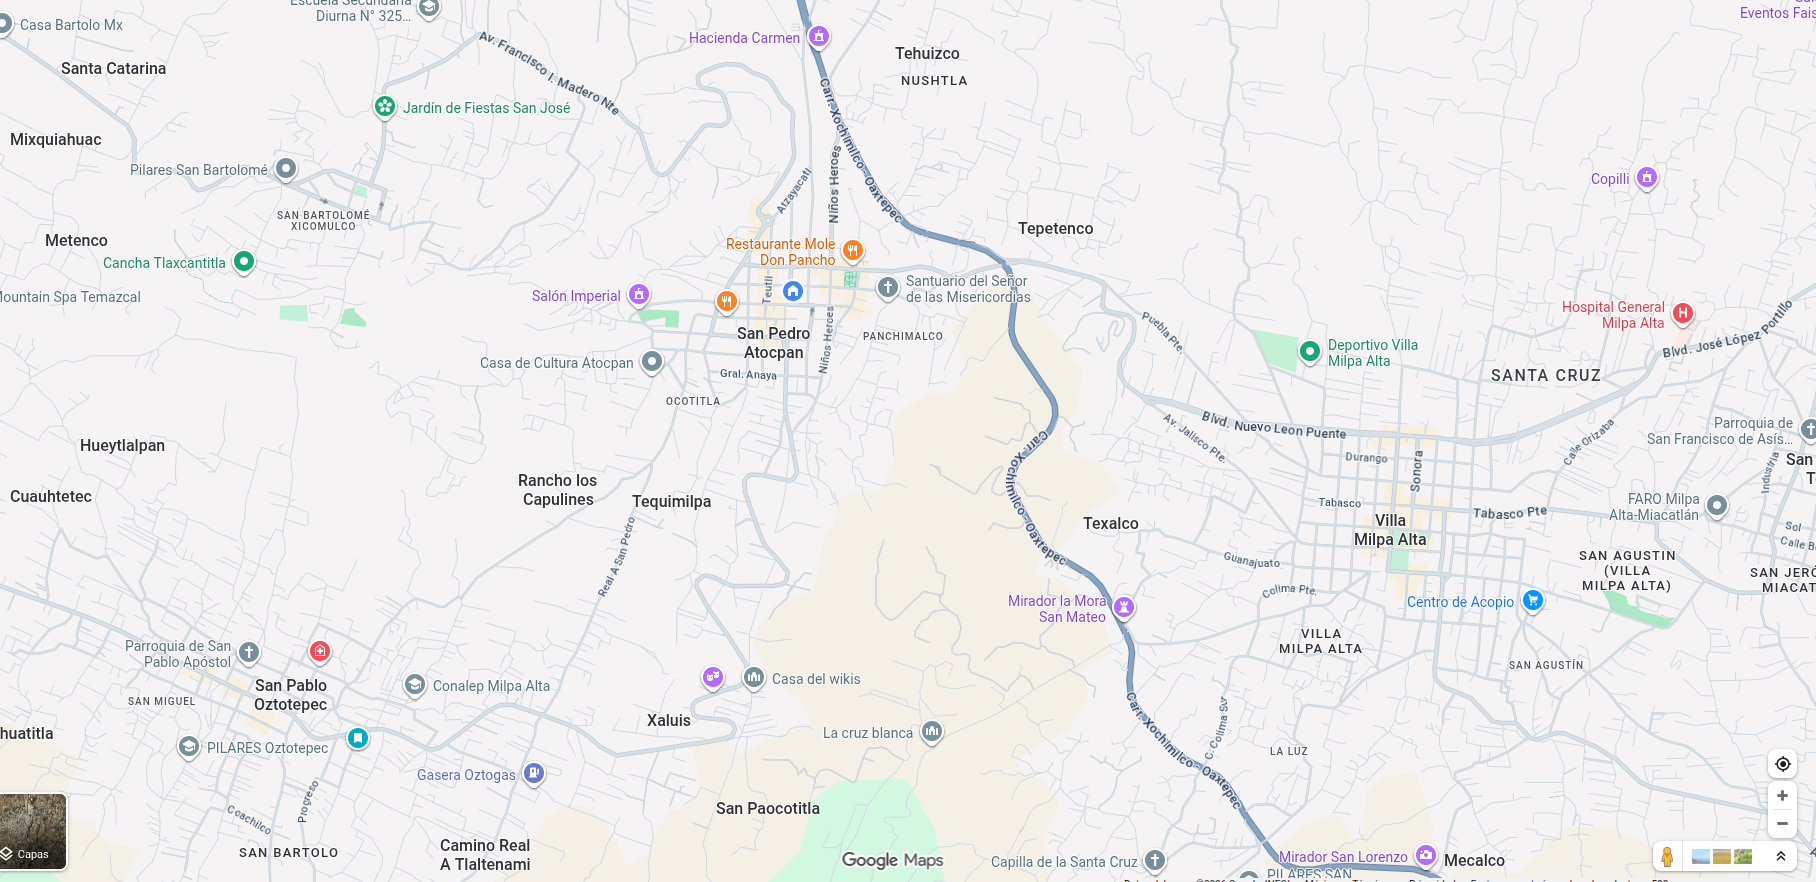
\includegraphics[width=\textwidth]{img/Planos/Ubicacion/Mapa1.png}
        \caption{Mapa general de San Pedro Atocpan: Colindancias con los pueblos de Milpa Alta y barreras geográficas de la Sierra Chichinautzin. Fuente: Google Maps.}
        \label{subfig:mapa-general}
    \end{subfigure}
    
    \vspace{0.4cm} % Espaciado elegante y controlado entre ambos planos
    
    % Segunda Subfigura (Abajo)
    \begin{subfigure}[b]{0.85\textwidth}
        \centering
        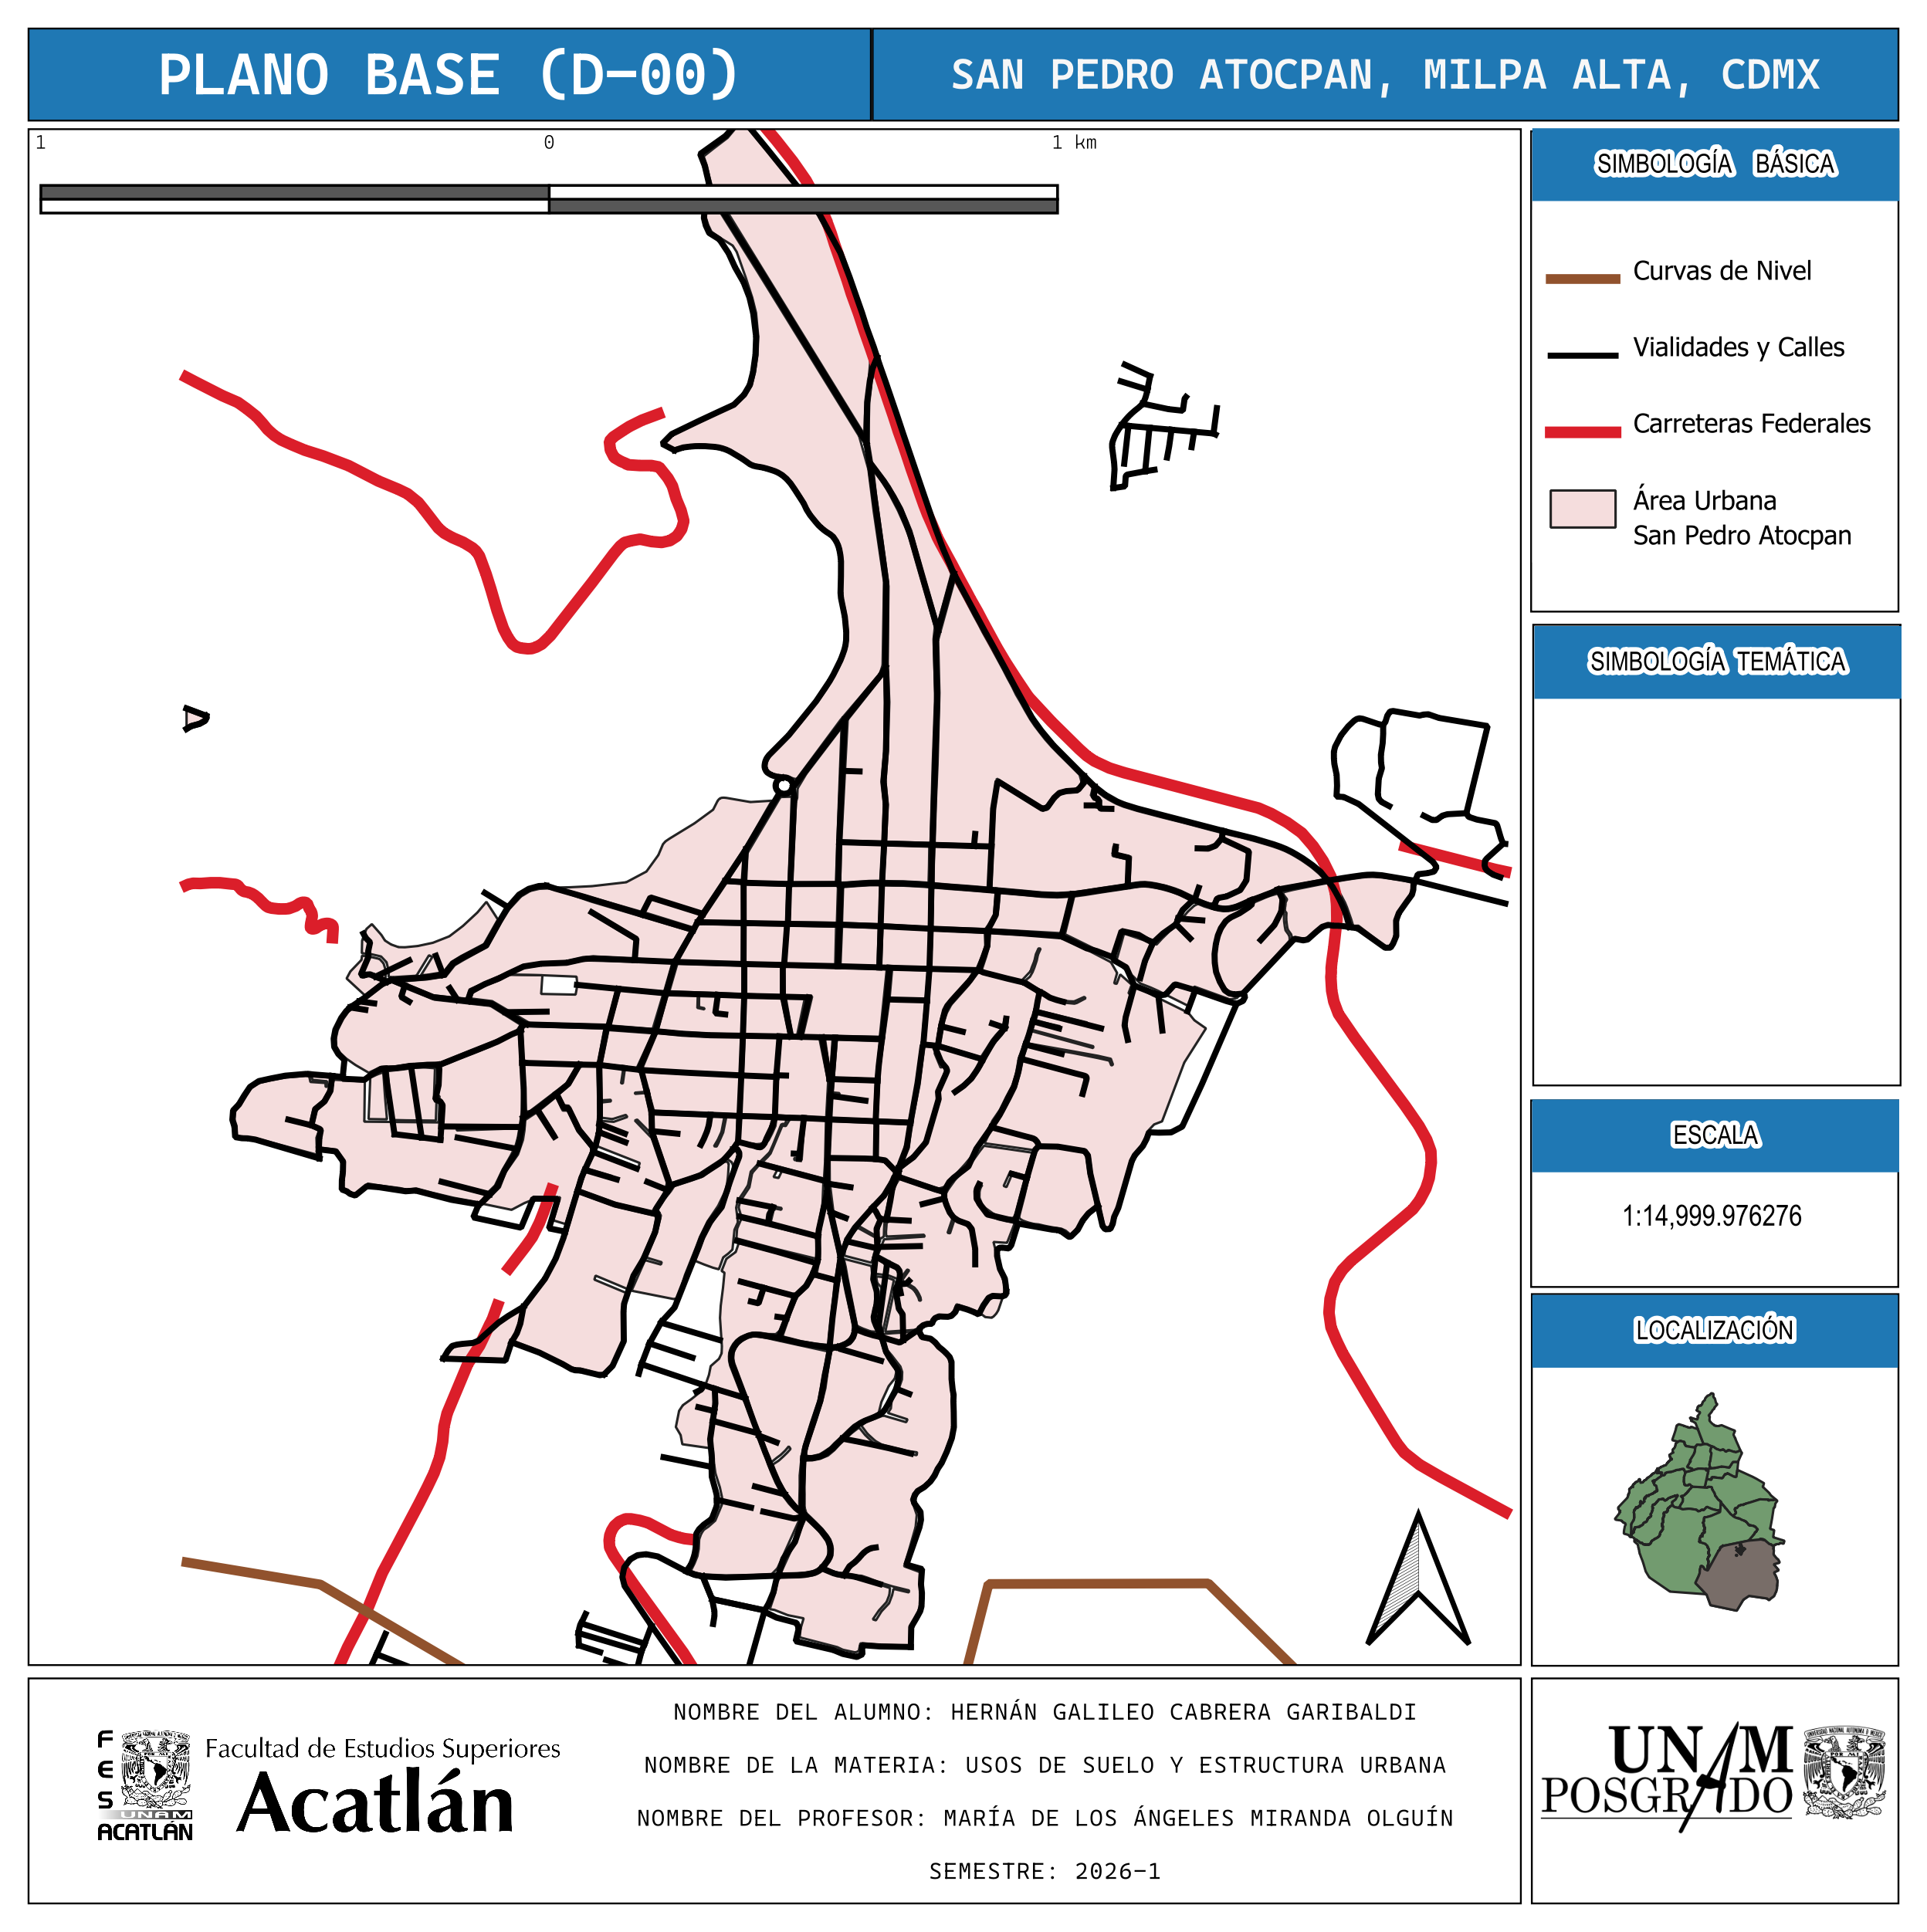
\includegraphics[width=\textwidth]{img/Planos/UsosDeSuelo/D-00.png}
        \caption{Mapa base urbano de San Pedro Atocpan. Fuente: Elaboración propia con datos de INEGI.}
        \label{subfig:contexto_general}
    \end{subfigure}
    
    % Título maestro unificado
    \caption{Ubicación geográfica, límites territoriales y marco cartográfico de referencia del área de estudio.}
    \label{fig:cartografia_referencia}
\end{figure}

\subsection{Sub-polígonos de Análisis Específico}
\label{ssec:subpoligonos-especificos}

Para un estudio detallado de la \termino{Puesta en Valor} y la mitigación de riesgos, se han categorizado 
tres áreas específicas que narran la evolución de la memoria y la función religiosa tras la 
tragedia acontecida en 1935.

\subsubsection{Polígono 1: Área de Afectación Crítica (Total)}
\label{subsubsec:poligono-afectacion-critica}

Este polígono representa el área de mayor daño histórico documentado. 
Integra el complejo religioso compuesto por el templo original de \termino{Yencuictlalpan} y el 
nuevo Santuario. Es el espacio donde la corriente de agua y lodo de 1935 concentró su 
fuerza destructiva \cite{excelsior1935zona}.

\begin{itemize}
    \item \textbf{Superficie:} 2,864.005 $m^2$.
    \item \textbf{Elementos clave:} Capilla de San Martín Caballero y 
            Templo del Señor de las Misericordias.
\end{itemize}

% Bloque de imagen: Plano Polígono 1
\begin{figure}[H]
    \centering
    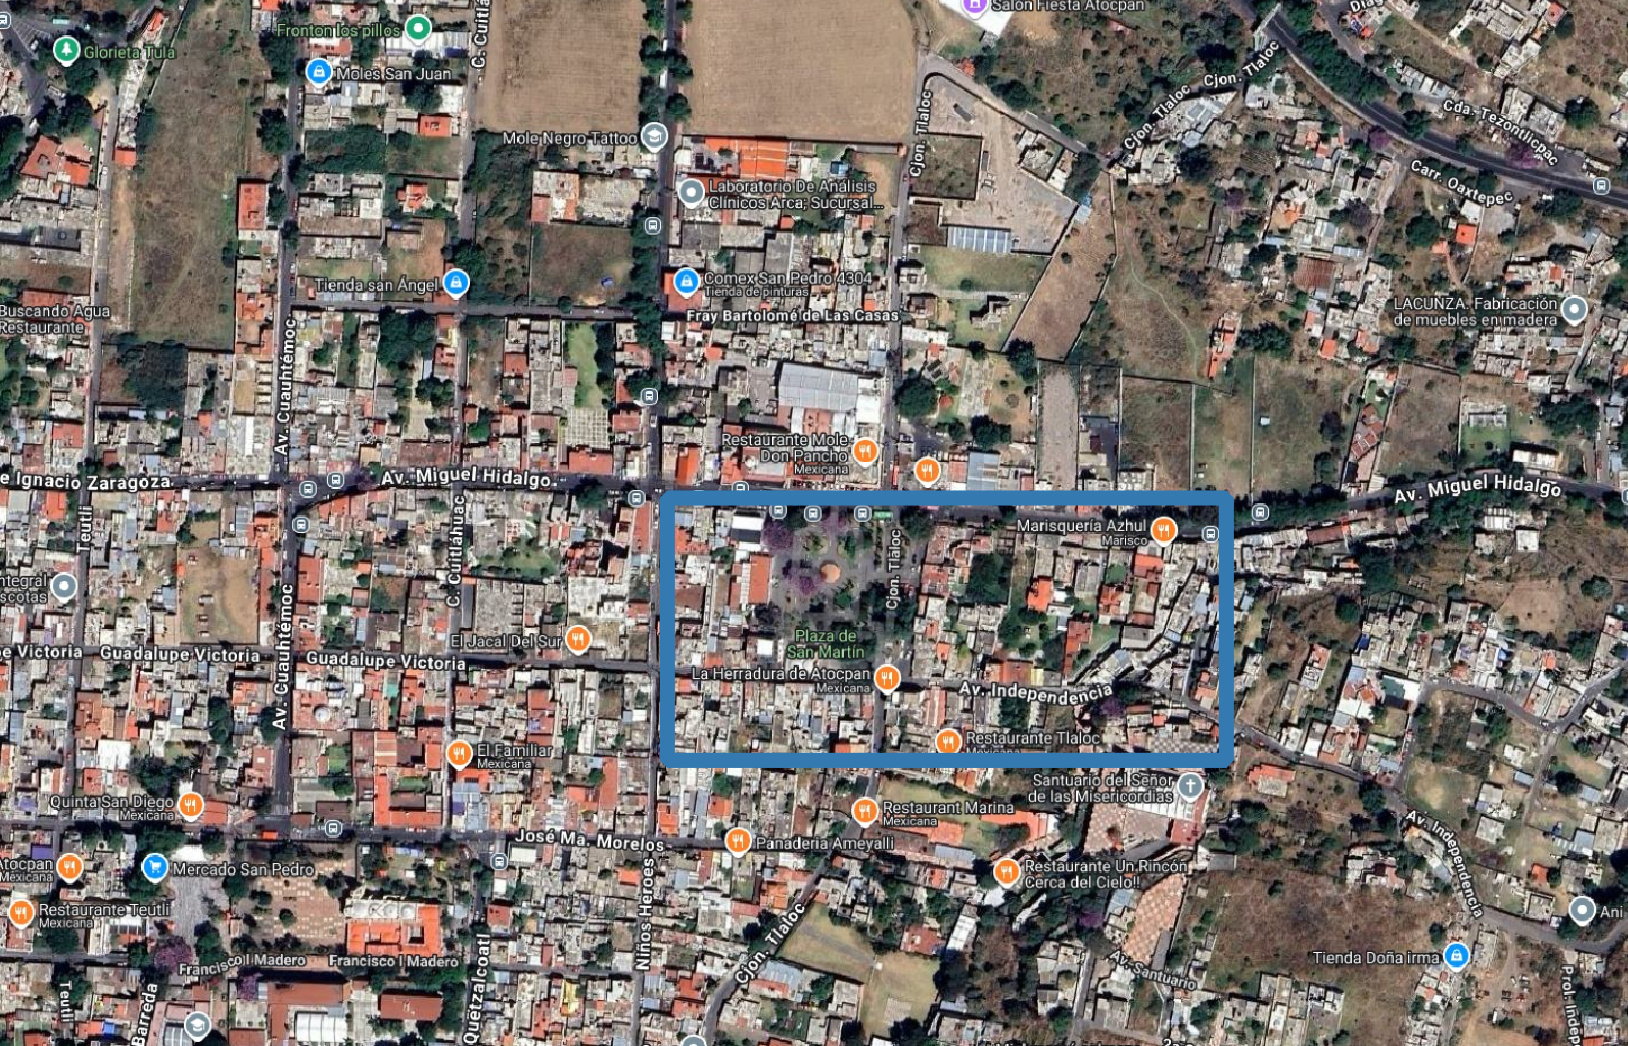
\includegraphics[width=0.8\textwidth]{img/Planos/Ubicacion/Poligono3.png}
    \caption{Plano de detalle del Polígono 1: Área de mayor daño estructural histórico. Fuente: Elaboración propia.}
    \label{fig:poligono_1}
\end{figure}

\subsubsection{Polígono 2: Recinto Histórico de \termino{Yencuictlalpan}}
\label{subsubsec:poligono-recinto-historico}

Corresponde al área original de la Capilla de \termino{Yencuictlalpan} (hoy San Martín Caballero). 
Este sitio es el epicentro de la memoria intangible de la comunidad, pues era el lugar donde 
se resguardaba la figura del Señor de las Misericordias en 1935 cuando ocurrió la inundación de 
2 metros de altura \cite{santuarioSFtesoro}.

\begin{itemize}
    \item \textbf{Superficie:} 5,709.348 $m^2$.
    \item \textbf{Relevancia:} Punto de origen de la resiliencia comunitaria y 
            reconstrucción post-desastre.
\end{itemize}

% Bloque de imagen: Plano Polígono 2
\begin{figure}[H]
    \centering
    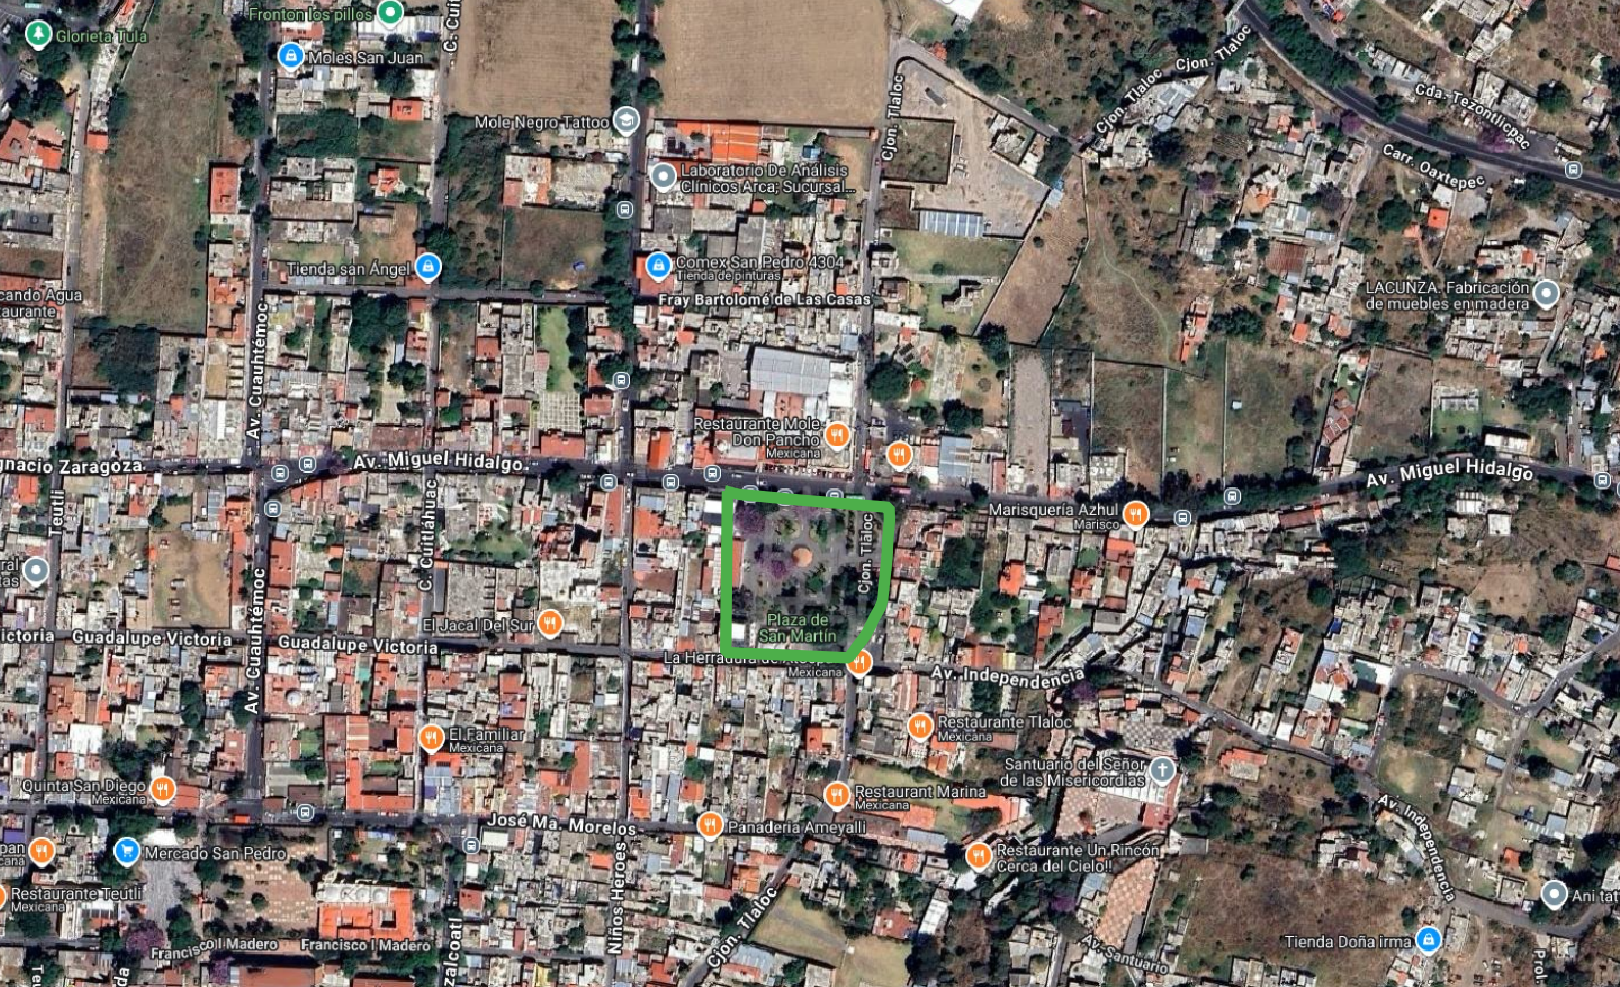
\includegraphics[width=0.8\textwidth]{img/Planos/Ubicacion/Poligono2.png}
    \caption{Plano de detalle del Polígono 2: Capilla original y sitio de la tragedia de 1935. 
            Fuente: Elaboración propia.}
    \label{fig:poligono_2}
\end{figure}

\subsubsection{Polígono 3: Santuario del Señor de las Misericordias}
\label{subsubsec:poligono-santuario-1960}
Área que comprende el templo moderno cuya construcción finalizó a finales de la década de 1960. 
Este edificio fue financiado mediante recursos comunales y aportaciones del pueblo, simbolizando 
la recuperación económica y espiritual de Atocpan tras el desastre hídrico \cite{santuarioSFtesoro}.
\begin{itemize}
    \item \textbf{Superficie:} 35,170.286 $m^2$.
    \item \textbf{Relevancia:} Lugar de descanso actual del cristo y centro de la feria 
        patronal contemporánea.
\end{itemize}

% Bloque de imagen: Plano Polígono 3
\begin{figure}[H]
    \centering
    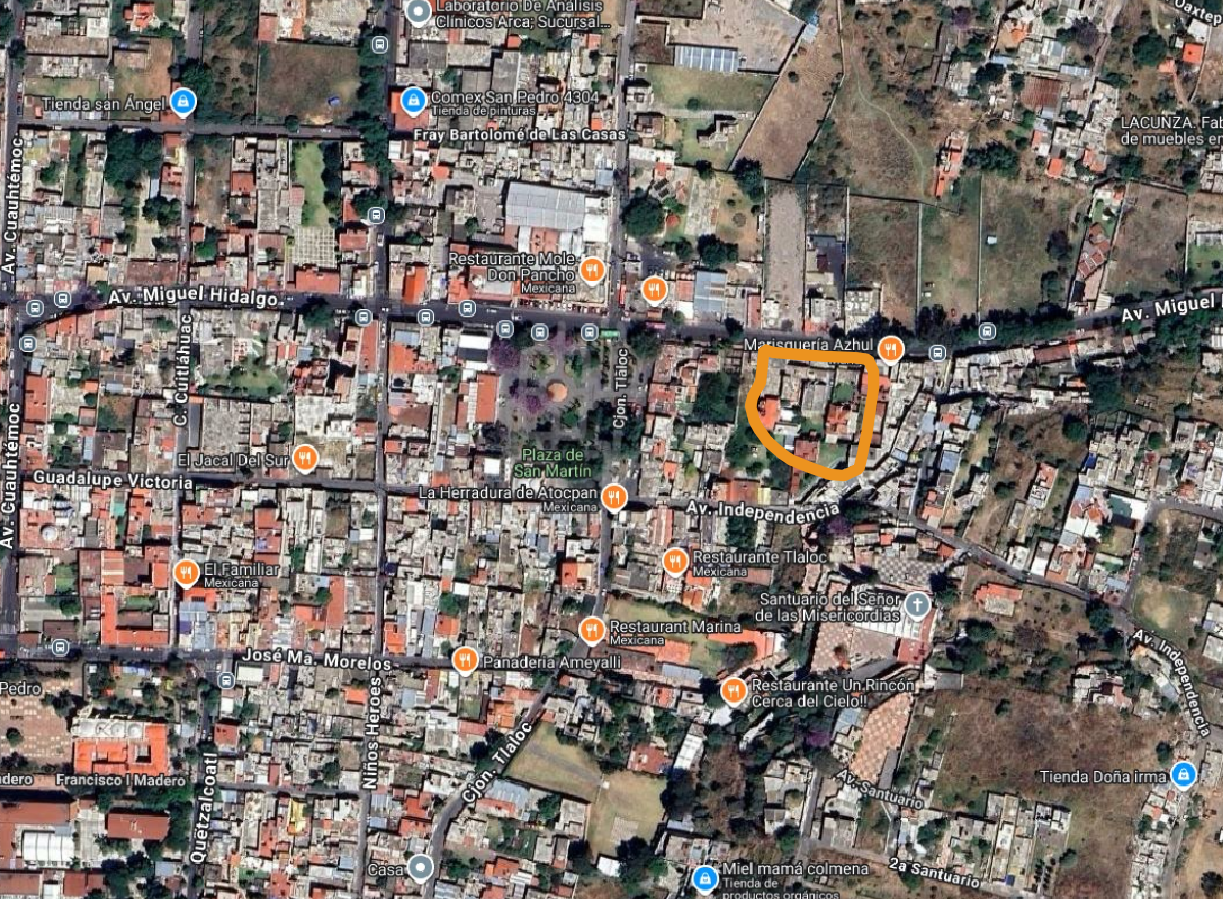
\includegraphics[width=0.8\textwidth]{img/Planos/Ubicacion/Poligono1.png}
    \caption{Plano de detalle del Polígono 3: Emplazamiento del Santuario moderno (década de 1960). 
    Fuente: Elaboración propia.}
    \label{fig:poligono_3}
\end{figure}

La delimitación espacial e interrelación física de las tres áreas analizadas evidencia que los polígonos 
no funcionan como células aisladas, sino como un sistema patrimonial y de riesgo hídrico integrado. 
Para una comprensión analítica integral de las dinámicas topográficas, las curvas de nivel y el 
comportamiento de escurrimientos vectorizados de la microcuenca sobre la traza del centro histórico, 
se puede consultar el \textbf{Anexo~\ref{anexo:cartografia}} (pág.~\pageref{anexo:cartografia}), 
el cual contiene el \textbf{Plano~\ref{fig:mapa_anexo_general}} procesado con las bases geoespaciales 
definitivas de este plan de regeneración.